\documentclass[10pt,a4paper,openbib]{article}
\usepackage[utf8]{inputenc}
\usepackage{amsmath}
\usepackage{amsfonts}
\usepackage{amssymb}
\usepackage{multicol}
\usepackage{graphicx}
\usepackage{caption}
\usepackage{subcaption}
\usepackage{mathtools}
\usepackage{natbib}
\usepackage{url}
\usepackage{float}
\usepackage{multirow}
\usepackage[margin=1.5cm]{geometry}
\author{Helen Harman, \\Aberystwyth University, \\heh14@aber.ac.uk,\\ Student Number: 110007212}
\title{Using Genetic Algorithms to Solve the Travelling Salesman Problem}

\newcommand{\subsubfloat}[2]{%
  \begin{tabular}{@{}c@{}}#1\\#2\end{tabular}%
}
\begin{document}

\maketitle

\section*{\vspace{-1.2cm} }

\begin{multicols}{2}
\section{Introduction}
The aim of the travelling salesman problem (TSP) is to find the shortest possible tour between cities. The tour must pass through all cities before returning to the starting city. The number of possible solutions is the factorial of the number of cities. For example 5 cities has 120 possible solutions, whereas 6 cities has 720 solutions. The TSP is NP-hard, and no general solution to solving it has been found. \cite{tspMathWorld}\\

\noindent The travelling salesman problem has been around since the 1930s. Initially it was known as the ``48 state problem". Hassler Whitney wanted to find the shortest school bus route between 49 cities across all 48 US states. By the mid 1940s the problem had been renamed to the travelling salesman problem. \cite{tspBackgroundWebsite} Though it is unclear as to who came up with the name. \\

\noindent In 1954 G. Dantzig et al. \cite{Dantzig} came up with a solution involving 49 cities. Since then solutions involving many more cities have been found. In 2004 D. Applegate et al. came up with a solution to 24,978 cities.\cite{milestonesWebsite}\\

\noindent For many of the solutions found artificial intelligence has been used. These methods include swam intelligence, neural networks, and Genetic Algorithms (GA). This report will look at solving the TSP using GAs.\\


\noindent GAs can be applied to large search problems. A initial population is generated that covers a large distribution of the search space. Based on how well these solutions, called individuals, perform the population is evolved in the hope that the individuals will converge on the optimal solution. The population is evolved using selection, crossover and mutation operations, these come under the umbrella term genetic operations.\\


\noindent There has been a lot of previous work in applying GAs to the TSP. This includes looking at the affect of using different crossover functions. Ahmed \cite{ahmed2010genetic} introduces a new crossover operator and compares this to previously used crossover operators. Their selection operator keeps the top individuals and is performed after the crossover operation. Abdoun et al. \cite{abdoun2012analyzing} compared the affect of different mutation operations; and uses roulette wheel selection. Both of these use a array containing a list of cities to represent the tour. \\

\noindent This report will compare the use of two different representations, and two selection operators. In section~\ref{design} the design decisions will be discussed; and section~\ref{Experiments} will discuss the different experiments that have been performed and their results.

\section{Design} \label{design}

\subsection{System Design}

The system has been designed to allow different genetic operations and representations to be easily changed. This is done through the use of abstract classes which take a generic type. An abstract class has been created for representations, the population, mutation operations, selection operations and crossover operations.  An example design for this is shown in figure~\ref{fig:classDiagram}. This allows different genetic operators and representations to be used without repeated code. \\

\begin{figure}[H]
\begin{center}
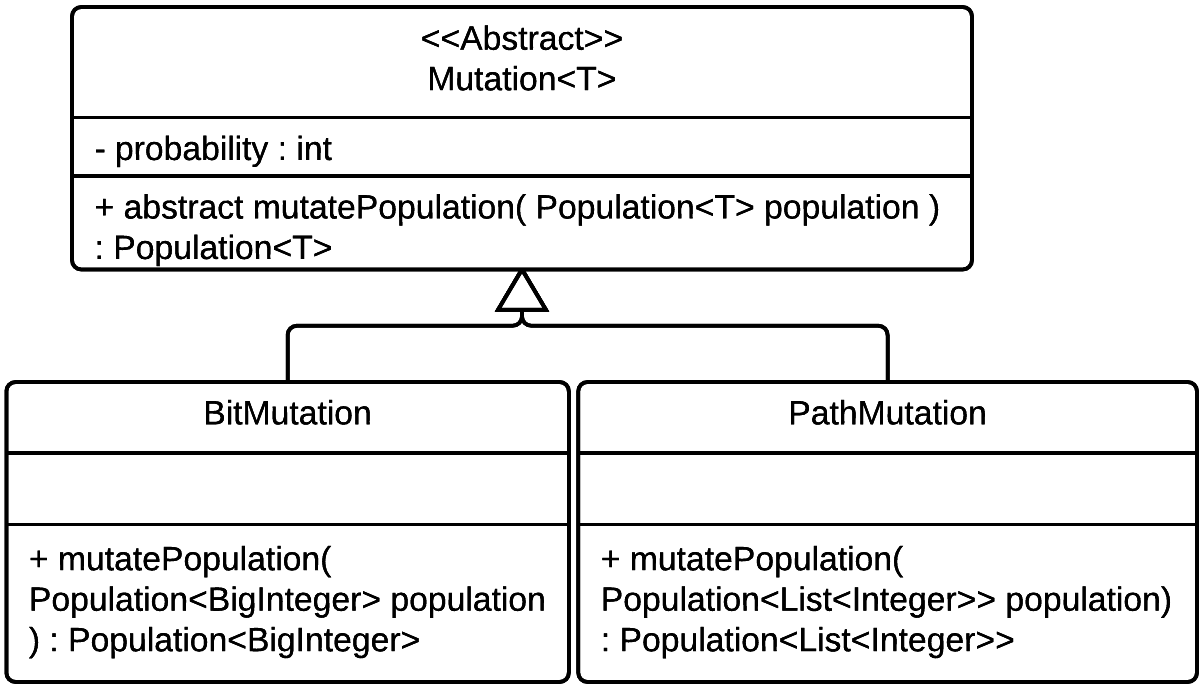
\includegraphics[scale=0.8]{images/classDiagram.png} 
\caption{UML class diagram for  the mutation operators}
\label{fig:classDiagram}
\end{center}
\end{figure}

\noindent Due to the object orientated nature of the design and the use of generic types I chose to use Java. A basic command line interface will be provided to allow the different parameters to be selected. An image showing the shortest found route will be produced. MLPlot \cite{mlPlot} will be used to produce graphs showing how the fitness varies between generations. \\

\noindent I chose to use binary representation (the details of this will be discussed in section~\ref{representation}). The initial plan was to use Java's BitSet class to hold hold this representation. To do this a long value would be used and converted into the BitSet. Each value represents a different solution, therefore 21 cities would cause a the long to overflow. The maximum value for a long is $2^{63}-1$ and there are $5.1*10^{19}$ possible solutions. Therefore, Java's BigInteger class is used. The BitInteger class allows for bitwise operations and can be treated as I binary or denary value. \\

\noindent The stopping criteria is based on how the average fitness changes across the generations. If the average fitness does not decrease for $N$ generations the GA will stop. N will be set to 10 for the experiments. It is expected that the average fitness may rise between some generations, therefore using 10 should give enough leeway for this to happen. I considered using the fittest individual within the stopping criteria, however it is likely that this may not change for several generations, which could cause the GA to converge prematurely.


\subsection{Representations} \label{representation}

A solution to the TSP can be encoded in many different ways. This includes as an ordered list of cities; a matrix of points; or as a binary value. There are advantages and disadvantages for each type of representation. \\

\noindent Binary representation was chosen as often this makes the mutation and crossover functions simpler and in other situations has led to better results than alternative representations. This will be compared to path representation, due to path representation being commonly used for the TSP.\\

%\noindent When using an ordered list of cities a check that the same city has not been visited twice should be performed. When doing the genetic operations, participially crossover, cities some cities may be repeated whereas others will not be visited. This causes extra computations to have to be performed. The use of binary representation removes this issue. \\

\noindent \textit{Path Representation} \\

\noindent The TSP can be represented as a list of cities in the order that they are visited. For example the list A,B,C,D,E means that city A is visited first followed by B then C and so on. The tour will start and end at city A.  This is known as path representation.\cite{abdoun2012analyzing} \\

\noindent \textit{Binary Representation}

\noindent Each binary value represents a different tour. As shown in table~\ref{table:binaryRep}, the tours are numbered in alphabetical order. The algorithm for translating between the representation is described by A. Mohebifar \cite{mohebifar2006new}. \\

\noindent The difference between the positions of the cities in an initial tour (e.g. ABCDE) and another tour can be calculated and transformed into binary. The inverse of this can be used to translate from binary to the order list. The algorithms for these are shown in figure ~\ref{fig:makeBinary} and \ref{fig:toPath} respectively.\\

\begin{figure}[H]
\begin{center}
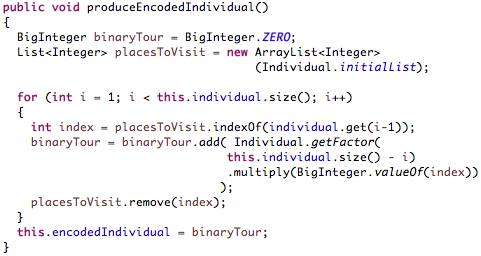
\includegraphics[scale=0.5]{images/makeBinary.png} 
\caption{How the binary representation of the individual is created from an ordered list of cities. }
\label{fig:makeBinary}
\end{center}
\end{figure}

\begin{figure}[H]
\begin{center}
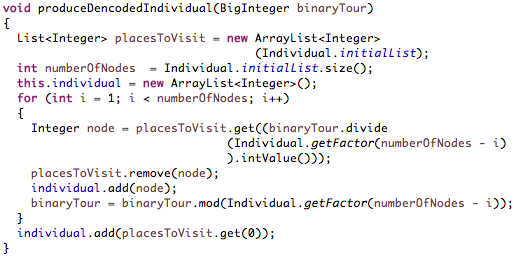
\includegraphics[scale=0.5]{images/makeOrderedList.png} 
\caption{How the order list of cities is created from the binary value.}
\label{fig:toPath}
\end{center}
\end{figure}


\begin{table}[H]
\centering
\begin{tabular}{|l|c|c|}
\hline
  & \multicolumn{1}{l|}{\textbf{Ordered tour}} & \multicolumn{1}{l|}{\textbf{Binary representation}} \\ \hline
1 & ABCDE                                      & 0000000                                             \\ \hline
2 & ABCED                                      & 0000001                                             \\ \hline
3 & ABDCE                                      & 0000010                                             \\ \hline
4 & ABDEC                                      & 0000011                                             \\ \hline
... & ...                                      & ...                                             \\ \hline
120 & EDCBA                                      & 1111000                                             \\ \hline
\end{tabular}
\caption{Binary representation of tours through cities A, B, C, D and E.}
\label{table:binaryRep}
\end{table}

\noindent The use of binary allows simple genetic operations to be used. However, the additional calculations needed to translate between binary and path representations may cause the GA to be computationally slower than using path representation.  \\


\noindent The results will discus and compare the fitness achieved by using binary and path representation. The genetic operators chosen must differ slightly between the two representations; but will be kept as similar as possible to allow a fair comparison to be performed.


\subsection{Genetic Operators} 

\subsubsection{Selection}

\textit{Multi-reserved strategy}\\

\noindent Often GAs will converge on a local minima causing them to return suboptimal results. The multi-reserved strategy tries to prevent this by taking the distance between the individuals into account, as well as the fitness, when performing selection. I have used the ideas presented in  \cite{IB_GA} and \cite{chen2008solving} to perform a multi-reserved strategy to solve the TSP. The algorithm can be described as :
\begin{itemize}
\item Selected the top k\% (eg. 10\%) of the population. (potential\_reserved\_list) 
	\begin{itemize}
	\item Stored the rest of the population in an unreserved\_list
	\end{itemize}
\item Add the fittest individual (B) to a reserved\_list
\item For each individual (I) in the potential\_reserved\_list:
	\begin{itemize}
	\item if $fitness(B)  - fitness(I) < a$ then add I to the reserved\_list
	\item else if $fitness(B)  - fitness(I) > b$ then add I to the unreserved\_list
	\item else if $dis(B, I) > c$ then add I to the reserved\_list
	\item else add I to the unreserved\_list
	\end{itemize}
\item Crossover and mutation will be applied to the two lists. The next generation will be formed of 50\% from the reserved\_list and 50\% from the unreserved\_list.
\item $k$, $a$, $b$ and $c$ are constants defined by the user.
\end{itemize}

\noindent Setting k too small could cause the population to not retain enough variation, but setting it to too high will allow more weaker individuals to be kept, which could cause the fitness to increase. These constants could have a large effect on the performance of the GA. \\

\noindent Tanimoto distance will be used for the binary representation. For path representation the distance will be calculated based on the difference between the indexes the cities appear in the two tours. \\

\noindent This method should allow the fittest individuals that a distributed across a large search space to be kept. The multi-reserved strategy will be compared to rank selection, which is more commonly used in GAs.\\

\noindent \textit{Rank selection} \\

\noindent In rank selection the fittest individual is the most likely to be picked, the next fittest is the second most likely to be picked and so on. Though it is not guaranteed, this should allow the next generation to be formed mostly from the fittest individuals and a few less fit individuals. Picking less fit individuals should allow a larger area of the search space to be covered. \cite{baker1985adaptive}\\

\noindent Table~\ref{table:rankSelection} shows the probability of an individual being picked when the population contains 6 individuals. 

\begin{table}[H]
\centering
\begin{tabular}{|c|c|}
\hline
\multicolumn{1}{|l|}{\textbf{Index}} & \multicolumn{1}{l|}{\textbf{Probability of being picked}} \\ \hline
0                                    & 11 / 35                                                   \\ \hline
1                                    & 9 / 35                                                    \\ \hline
2                                    & 7 / 35                                                    \\ \hline
3                                    & 5 / 35                                                    \\ \hline
4                                    & 2 / 35                                                    \\ \hline
5                                    & 1 / 35                                                    \\ \hline
\end{tabular}
\caption{Rank selection : probability of an individual being picked. The individual at index 0 is the fittest indivdual and index 5 contains the least fit individual.}
\label{table:rankSelection}
\end{table}

\noindent Using rank selection may cause the next generation to only contain combinations of the fittest individuals, of the current population. This would lead to only a small area of the search space being evaluated, which is likely to result in a local minim being discovered. \\

\noindent However, preforming a random amount of crossover and mutation should allow a diverse population to be created. The next sections will introduce the crossover and mutation operations that are being used.


\subsubsection{Crossover} \label{crossoverExplained}

Consideration was also given to many types of crossover operations, this includes N-Point crossover, edge recombination crossover and sequential constructive crossover.\cite{ahmed2010genetic} As the focus of the experiments will be on the selection and representation used, a standard one-point crossover is applied. \cite{poli1998schema}  The following algorithm describes how crossing individual X with individual Y works : \\
\begin{itemize}
\item Generate a random number ($r$) between $0$ and probability ($c$) $*$ length of individual ($l$)
\item if $r < l$ then crossover is performed :
	\begin{itemize}
	\item swap each item in X, with each item in Y: who's position is less than r 
	\end{itemize}
\end{itemize}

\noindent \textit{Binary representation} \\

\noindent For binary representation crossover is performed by swapping the bits and checking that the binary value produced is less than the maximum number of solutions. 

\begin{figure}[H]
\begin{center}
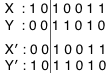
\includegraphics[scale=0.6]{images/binaryCrossover.png} 
\caption{Example of binary crossover}
\label{fig:binaryCrossover}
\end{center}
\end{figure}


\noindent \textit{Path Representation} \\

\noindent Performing crossover on order lists of cities may cause cities to be visited multiple times. Thus producing on invalid solution. A check is performed to find any cities that a missing from the list. Any repeated cities are replaced by missing cities. \\

\begin{figure}[H]
\begin{center}
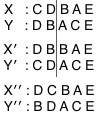
\includegraphics[scale=0.6]{images/orderCrossover.png} 
\caption{Example of crossover for path representation}
\label{fig:orderCrossover}
\end{center}
\end{figure}

\subsubsection{Mutation}\label{mutationExplained}

In order to stop all individuals from converging to the same value; and to widen the covered search area mutation is applied. Mutation that has a small effect on the individual will allow for local search; and large effects will allow individuals to escape local minimas. \\

\noindent For both binary and path representation a low mutation probability is used. This will cause a small percentage of the individuals to change. The amount of change the individual undergoes will be discussed separately for the two types of representation. \\

\noindent \textit{Binary Representation} \\

\noindent Commonly when mutating binary values a single probability is used to determine if an a independent bit within the individual should be flipped. However, in this situation the more significant a bit is the larger effect it has on the tour. \\


\noindent Therefore, the least significant bit has a $1/(p*1)$ probability of being mutated and the n-th bit has a $1/(p*n)$  chance of mutation. This will still allow large changes in the tour to take place, but this will rarely occur. \\

\noindent Consideration was given to just adding 1 to the binary value. This would allow the tour to change by a very small amount. However, including larger changes allows local minimals to be escaped. \\

\noindent \textit{Path Representation} \\

\noindent Mutating the order list of cities is performed using a much simpler method. Two cities within the individual are swapped. This causes a significant change in the tour being performed and should allow the exploration of a large distribution of the search space. Their is a $1/p$ probability of an individual being mutated. This will allow the majority of individuals to not be mutated, therefore information from previous generations will be retained.

\section{Experiments} \label{Experiments}

The section will explain the different experiments performed. The results will be presented and the differences between the results for the two representations and two selection operation will be discussed.


\subsection{Set-up}

\noindent The randomly generated cities will be spread across a 200 by 200 pixel sized area. The initial population will also be randomly generated. The initial population will remain the same for all experiments involving a number of cities. \\

\noindent Due to the indeterministic aspects of the GAs each experiment will be run 10 times and the average fitness will be calculated. This coupled with the use of the same population for each experiment should allow for a fair evaluation of the different approaches. \\


\subsection{Results}

The result tables contain : 
\begin{itemize}
\item Representation(Rep.) of the individuals either binary representation (B.) or path representation (P.) 
\item Selection (Sel.) used will either be Rank selection or the multi-reserved strategy (MRS).
\item Number of generations(Gen.) 
\item The average (Avg.) fitness of the final generation 
\item The fitness of the least fittest individual from the finial generation (least)
\item The fitness of the fittest (F.) individual from the finial generation 
\item The fitness of the fittest (F.) individual over all generations
\end{itemize}  

\subsubsection{Initial Experiments}

Some initial experiments were performed to determine what mutation and crossover probability should be used when comparing the representations, and selection operators. \\

\noindent \textit{Crossover probability} \\

% Please add the following required packages to your document preamble:
% \usepackage{multirow}
\begin{table}[H]
\centering
\begin{tabular}{|c|c|c|c|}
\hline
\multicolumn{1}{|l|}{\textbf{Crossover}} & \multicolumn{1}{l|}{\textbf{Rep.}} & \multicolumn{1}{l|}{\textbf{Sel.}} & \multicolumn{1}{l|}{\textbf{Fittest}} \\ \hline
\multirow{4}{*}{5}                       & \multirow{2}{*}{B.}                & Rank                               & 973                                   \\ \cline{3-4} 
                                         &                                    & MRS                                & 1035                                  \\ \cline{2-4} 
                                         & \multirow{2}{*}{P.}                & Rank                               & 765                                   \\ \cline{3-4} 
                                         &                                    & MRS                                & 754                                   \\ \hline
\multirow{4}{*}{10}                      & \multirow{2}{*}{B.}                & Rank                               & 948                                   \\ \cline{3-4} 
                                         &                                    & MRS                                & 1021                                  \\ \cline{2-4} 
                                         & \multirow{2}{*}{P.}                & Rank                               & 748                                   \\ \cline{3-4} 
                                         &                                    & MRS                                & 782                                   \\ \hline
\multirow{4}{*}{15}                      & \multirow{2}{*}{B.}                & Rank                               & 986                                   \\ \cline{3-4} 
                                         &                                    & MRS                                & 1055                                  \\ \cline{2-4} 
                                         & \multirow{2}{*}{P.}                & Rank                               & 756                                   \\ \cline{3-4} 
                                         &                                    & MRS                                & 772                                   \\ \hline
\multirow{4}{*}{20}                      & \multirow{2}{*}{B.}                & Rank                               & 1011                                  \\ \cline{3-4} 
                                         &                                    & MRS                                & 1026                                  \\ \cline{2-4} 
                                         & \multirow{2}{*}{P.}                & Rank                               & 751                                   \\ \cline{3-4} 
                                         &                                    & MRS                                & 762                                   \\ \hline
\end{tabular}
\caption{Fittest tour found when using different crossover probabilities. The meaning of these crossover values have been described in section~\ref{crossoverExplained}.}
\label{table:crossover20cities}
\end{table}

\noindent After running the GAs on different crossover probabilities, it was decided that a probability of 10 will be used during the rest of the experiments. The fitness of the fittest individual starts to rise when a value greater than 10 is used. (Shown in table~\ref{table:crossover20cities} )\\

\noindent \textit{Mutation probability} \\

\noindent 500 will be used for the mutation probability. A greater or lesser value during the initial experiments caused, on average, a longer tour to be found. Two much mutation causes the generations to lose good information, whereas, too little mutation and individuals will not be able to escape local minimas. \\

% Please add the following required packages to your document preamble:
% \usepackage{multirow}
\begin{table}[H]
\centering
\begin{tabular}{|c|c|c|c|}
\hline
\multicolumn{1}{|l|}{\textbf{Mutation}} & \multicolumn{1}{l|}{\textbf{Rep.}} & \multicolumn{1}{l|}{\textbf{Sel.}} & \multicolumn{1}{l|}{\textbf{Fittest}} \\ \hline
\multirow{4}{*}{400}                    & \multirow{2}{*}{B.}                & Rank                               & 1132                                  \\ \cline{3-4} 
                                        &                                    & MRS                                & 1201                                  \\ \cline{2-4} 
                                        & \multirow{2}{*}{P.}                & Rank                               & 830                                   \\ \cline{3-4} 
                                        &                                    & MRS                                & 845                                   \\ \hline
\multirow{4}{*}{450}                    & \multirow{2}{*}{B.}                & Rank                               & 1155                                  \\ \cline{3-4} 
                                        &                                    & MRS                                & 1213                                  \\ \cline{2-4} 
                                        & \multirow{2}{*}{P.}                & Rank                               & 817                                   \\ \cline{3-4} 
                                        &                                    & MRS                                & 855                                   \\ \hline
\multirow{4}{*}{500}                    & \multirow{2}{*}{B.}                & Rank                               & 1103                                  \\ \cline{3-4} 
                                        &                                    & MRS                                & 1182                                  \\ \cline{2-4} 
                                        & \multirow{2}{*}{P.}                & Rank                               & 800                                   \\ \cline{3-4} 
                                        &                                    & MRS                                & 853                                   \\ \hline
\multirow{4}{*}{550}                    & \multirow{2}{*}{B.}                & Rank                               & 1135                                  \\ \cline{3-4} 
                                        &                                    & MRS                                & 1140                                  \\ \cline{2-4} 
                                        & \multirow{2}{*}{P.}                & Rank                               & 868                                   \\ \cline{3-4} 
                                        &                                    & MRS                                & 897                                   \\ \hline
\multirow{4}{*}{600}                    & \multirow{2}{*}{B.}                & Rank                               & 1142                                  \\ \cline{3-4} 
                                        &                                    & MRS                                & 1190                                  \\ \cline{2-4} 
                                        & \multirow{2}{*}{P.}                & Rank                               & 864                                   \\ \cline{3-4} 
                                        &                                    & MRS                                & 894                                   \\ \hline
\end{tabular}
\caption{Fittest tour found when using different mutation probabilities. The meaning of these values have been described in section~\ref{mutationExplained}.}
\label{table:mutation20cities}
\end{table}

\subsubsection{Representation and Selection Experiments}
The experiments comparing binary representation to path representation, and multi-reserved strategy to rank selection, were performed using a range of different amounts of cities. The first of these will look at 10 cities being used. \\

\noindent \textit{10 cities}\\

\noindent When the multi-reserved strategy is used, with either representations, a much higher least fittest value is seen for the final generation. Due to the genetic operations the least fittest individual changes considerably between generations. (Figures~\ref{fig:cities10GraphBinaryfalse} to \ref{fig:cities10GraphPathtrue}). Therefore, it is likely that these experiments have coincidently converged on a higher least fittest, in comparison to rank selection. \\

\begin{table}[H]
\centering
\begin{tabular}{|c|c|c|c|c|c|c|}
\hline
\multicolumn{1}{|l|}{\multirow{2}{*}{\textbf{Rep.}}} & \multicolumn{1}{l|}{\multirow{2}{*}{\textbf{Sel.}}} & \multicolumn{1}{l|}{\multirow{2}{*}{\textbf{Gen.}}} & \multicolumn{3}{c|}{\textbf{In final generation}}                                                                & \multicolumn{1}{l|}{\multirow{2}{*}{\textbf{F.}}} \\ \cline{4-6}
\multicolumn{1}{|l|}{}                               & \multicolumn{1}{l|}{}                               & \multicolumn{1}{l|}{}                               & \multicolumn{1}{l|}{\textbf{Avg.}} & \multicolumn{1}{l|}{\textbf{Least}} & \multicolumn{1}{l|}{\textbf{F.}} & \multicolumn{1}{l|}{}                                  \\ \hline
\multirow{2}{*}{B.}                                  & Rank                                                &513                                                  & 544                                & 637                                 & 541                                   & 541                                                    \\ \cline{2-7} 
                                                     & MRS                                                & 694                                                 & 559                                & 787                                 & 533                                   & 533                                                    \\ \hline
\multirow{2}{*}{P.}                                  & Rank                                                & 54                                                  & 534                                & 534                                 & 534                                   & 633                                                    \\ \cline{2-7} 
                                                     & MRS                                                & 62                                                  & 534                               & 607                                 & 531                                   & 531                                                    \\ \hline
\end{tabular}
\caption{Number of cities : 10, Population size : 100}
\label{table:10cities}
\end{table}



\begin{figure}[H]
\begin{center}
    \begin{subfigure}[b]{0.15\textwidth}
        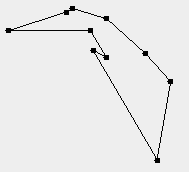
\includegraphics[width=\textwidth]{images/result1/Binaryfalse2.png}
        \caption{Solution found during many of the experiments.}
        \label{fig:cities10Many}
    \end{subfigure}
    \begin{subfigure}[b]{0.15\textwidth}
        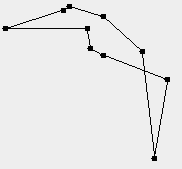
\includegraphics[width=\textwidth]{images/result1/Pathfalse4.png}
        \caption{Path \\representation using rank selection}
        \label{fig:10citiesPathFalseTour}
    \end{subfigure}
    \begin{subfigure}[b]{0.15\textwidth}
        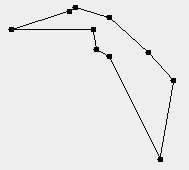
\includegraphics[width=\textwidth]{images/result1/Pathtrue7.png}
        \caption{Path \\representation \\using MRS}
        \label{fig:10citiesPathFalseTour}
    \end{subfigure}
    \caption{A selection of different best tours found from when using 10 cities.}
    \label{fig:10citiesTours}
\end{center}
\end{figure}


\noindent For many of the runs, the different experiments resulted in the same tour being found (figure~\ref{fig:cities10Many}). However, this is not the shortest tour possible. From figure~\ref{fig:cities10GraphBinaryfalse} and ~\ref{fig:cities10GraphBinarytrue} it is clear that the average and fittest fitnesses have decreased before then levelling off. Which provides evidence that a local minim has been reached.

\begin{figure}[H]
\begin{center}
        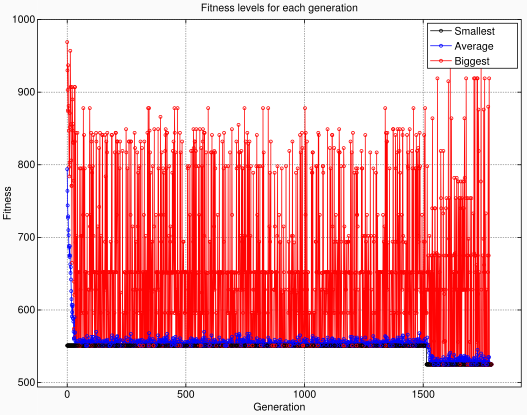
\includegraphics[width=0.45\textwidth]{images/result1/GraphBinaryfalse2.png}
        \caption{Binary representation using rank selection. This experiment resulted in the tour shown in figure~\ref{fig:cities10Many}.}
        \label{fig:cities10GraphBinaryfalse}
\end{center}
\end{figure}

\begin{figure}[H]
\begin{center}
        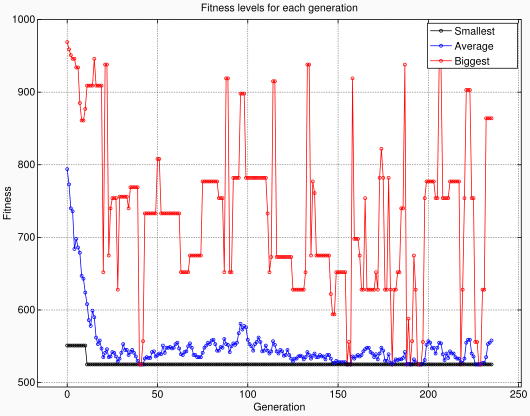
\includegraphics[width=0.45\textwidth]{images/result1/GraphBinarytrue1.png}
        \caption{Binary representation using MRS. This experiment resulted in the tour shown in figure~\ref{fig:cities10Many}.}
        \label{fig:cities10GraphBinarytrue}
\end{center}
\end{figure} 


\begin{figure}[H]
\begin{center}
        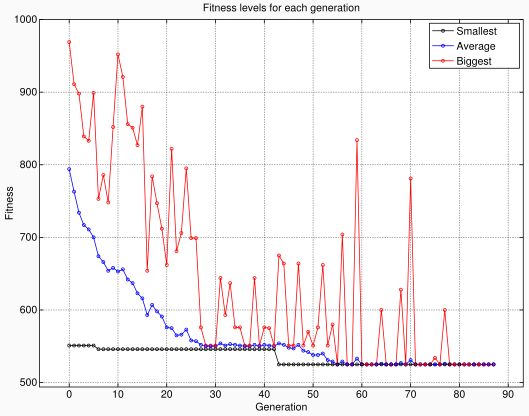
\includegraphics[width=0.45\textwidth]{images/result1/GraphPathfalse4.png}
        \caption{Path representation using rank selection.}
        \label{fig:cities10GraphPathfalse}
\end{center}
\end{figure}

\begin{figure}[H]
\begin{center}
        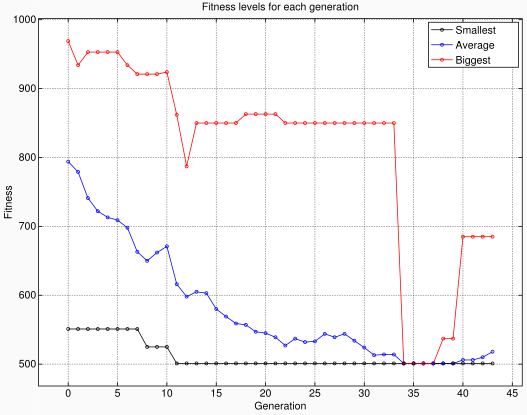
\includegraphics[width=0.45\textwidth]{images/result1/GraphPathtrue7.png}
        \caption{Path representation using MRS}
        \label{fig:cities10GraphPathtrue}
\end{center}
\end{figure} 

\noindent The path representation with rank selection has converged to a longer tour than the other experiments. As the average fitness has levelled off (figure~\ref{fig:cities10GraphPathfalse}) it is likely that a local minima has been researched. A possible reasons for this is that not enough variation and mutation occurred in order to search a wide distribution of the search space. With an average of only 54 generations, this experiment converged much quicker than the other experiments; potentially causing a smaller area of the search space to be covered. \\ 

\noindent Their is only a small difference in the fitness of the fittest individual for the multi-reserved strategy experiments (table~\ref{table:10cities}). Path representation using the multi-reserved strategy appears to, on average, find a fitter individual. However, as such a small difference is seen further experiments are need to see if this holds true for a greater number of cities. \\


\noindent \textit{15 cities} \\


\begin{figure}[H]
\begin{center}
    \begin{subfigure}[b]{0.24\textwidth}
    \begin{minipage}{\textwidth}\footnotesize

  		\subsubfloat{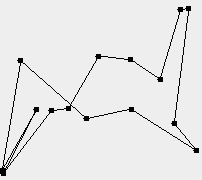
\includegraphics[width=0.48\textwidth]{images/result2/Binaryfalse6.png}}{Rank selection}\label{fig:cities15toursBR}
  		\subsubfloat{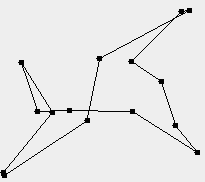
\includegraphics[width=0.48\textwidth]{images/result2/Binarytrue0.png}}{MRS}\label{fig:cities15toursOM}
 	\caption{Binary representation}\label{fig:cities15toursB}
  \end{minipage}
        
    \end{subfigure}
    \begin{subfigure}[b]{0.24\textwidth}
    \begin{minipage}{\textwidth}\footnotesize

  		\subsubfloat{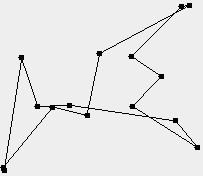
\includegraphics[width=0.48\textwidth]{images/result2/Pathfalse2.png}}{Rank selection}\label{fig:cities15toursOR}
  		\subsubfloat{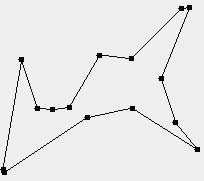
\includegraphics[width=0.48\textwidth]{images/result2/Pathtrue6.png}}{MRS}\label{fig:cities15toursOM}
 		\caption{Path representation}\label{fig:cities15toursO}
  \end{minipage}
        
    \end{subfigure} 
    \caption{Selection of tours produced for 15 cities}
    \label{fig:cities15tours}
\end{center}
\end{figure}


\noindent On average when using 15 cities, path representation has converged on a shorter tour than binary representation. The path representation which uses multi-reserved strategy results in the shortest found tour. \\


\begin{table}[H]
\centering
\begin{tabular}{|c|c|c|c|c|c|c|}
\hline
\multicolumn{1}{|l|}{\multirow{2}{*}{\textbf{Rep.}}} & \multicolumn{1}{l|}{\multirow{2}{*}{\textbf{Sel.}}} & \multicolumn{1}{l|}{\multirow{2}{*}{\textbf{Gen.}}} & \multicolumn{3}{c|}{\textbf{In final generation}}                                                                & \multicolumn{1}{l|}{\multirow{2}{*}{\textbf{F.}}} \\ \cline{4-6}
\multicolumn{1}{|l|}{}                               & \multicolumn{1}{l|}{}                               & \multicolumn{1}{l|}{}                               & \multicolumn{1}{l|}{\textbf{Avg.}} & \multicolumn{1}{l|}{\textbf{Least}} & \multicolumn{1}{l|}{\textbf{F.}} & \multicolumn{1}{l|}{}                                  \\ \hline
\multirow{2}{*}{B.}                                  & Rank                                                & 3426                                                & 870                                & 1538                                & 855                                   & 838                                                    \\ \cline{2-7} 
                                                     & MRS                                                & 1796                                                & 916                                & 1692                                & 842                                   & 842                                                    \\ \hline
\multirow{2}{*}{P.}                                  & Rank                                                & 118                                                  & 833                                & 982                                & 831                                   & 822                                                    \\ \cline{2-7} 
                                                     & MRS                                                & 282                                                 & 783                                & 1080                                & 771                                   & 771                                                    \\ \hline
\end{tabular}
\caption{Number of cities : 15, Population size : 200}
\label{my-label}
\end{table}

\begin{figure}[H]
\begin{center}
        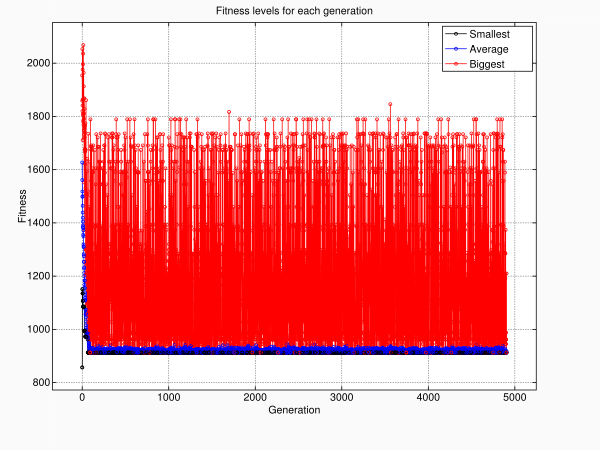
\includegraphics[width=0.45\textwidth]{images/result2/GraphBinaryfalse6.png}
        \caption{Binary representation using rank selection.}
        \label{fig:cities15GraphBinaryfalse}
\end{center}
\end{figure}

\begin{figure}[H]
\begin{center}
        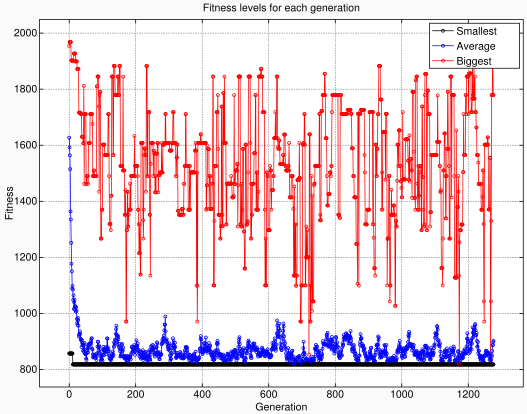
\includegraphics[width=0.45\textwidth]{images/result2/GraphBinarytrue0.png}
        \caption{Binary representation using MRS}
        \label{fig:cities15GraphBinarytrue}
\end{center}
\end{figure}


\begin{figure}[H]
\begin{center}
        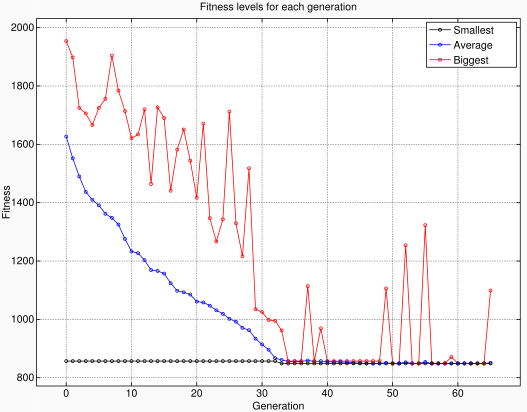
\includegraphics[width=0.45\textwidth]{images/result2/GraphPathfalse2.png}
        \caption{Path representation using rank selection.}
        \label{fig:cities15GraphPathfalse}    
\end{center}
\end{figure}

\begin{figure}[H]
\begin{center}
        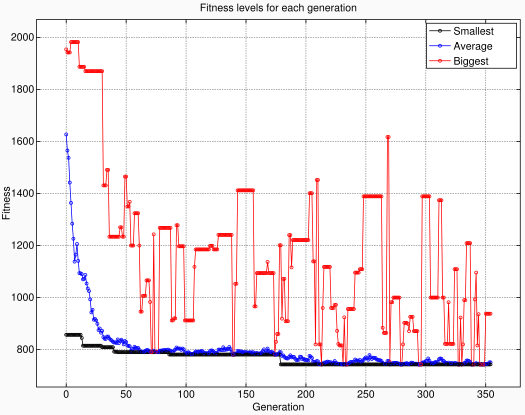
\includegraphics[width=0.45\textwidth]{images/result2/GraphPathtrue6.png}
        \caption{Path representation using MRS}
        \label{fig:cities15GraphPathtrue}
\end{center}
\end{figure}

\noindent it was predicted that the multi-reserved strategy would take more generations to converge. The distance between individuals is taken into account when performing this selection. Therefore, individuals with a lower fitness are more likely to be kept than when rank selection is used. This should allow a larger search space to be explored. However, binary representation using rank selection takes more generations to converge. Putting an even higher weighting on the elite individuals may allow this to converge using fewer generations. \\

\noindent When using the multi-reserved strategy the least fit individual is significantly higher than when rank selection is used. 50\% of the population is made from the non-reserved list, therefore there is a very high chance that an unfit individual will make it into the next generation.\\

\noindent When only 15 cities are used there is still very little difference between 3 of the average fittest individual's fitness. However, the path representation using multi-reserved strategy, on average, has given the shortest tour. Adding more cities will hopefully cause more variation within the results.\\

\noindent \textit{18 cities} \\

\noindent As we increase the number of cities to 18 it becomes clearer from both the resulting tours (figures~\ref{fig:cities18GraphBinary} and~\ref{fig:cities18GraphPath}) and the average results (table~\ref{table:18cities}) that the path representation results in a shorter tour being found.

\begin{figure}[H]
\begin{center}
    \begin{subfigure}[b]{0.23\textwidth}
        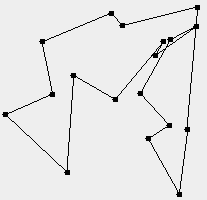
\includegraphics[width=0.48\textwidth]{images/result3/Binaryfalse0.png}
        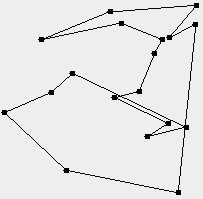
\includegraphics[width=0.48\textwidth]{images/result3/Binaryfalse7.png}
        \caption{Rank selection.}
        \label{fig:cities18GraphBinaryfalse}
    \end{subfigure}
    \begin{subfigure}[b]{0.23\textwidth}
        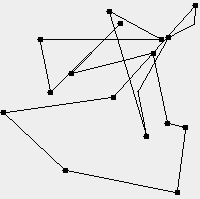
\includegraphics[width=0.48\textwidth]{images/result3/Binarytrue0.png}
        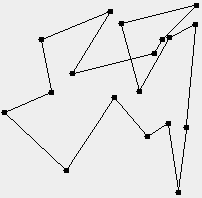
\includegraphics[width=0.48\textwidth]{images/result3/Binarytrue6.png}
        \caption{MRS}
        \label{fig:cities18GraphBinarytrue}
    \end{subfigure}  
    \caption{Binary representation}
    \label{fig:cities18GraphBinary}
\end{center}
\end{figure}




\begin{figure}[H]
\begin{center}
    \begin{subfigure}[b]{0.23\textwidth}
        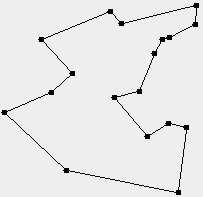
\includegraphics[width=0.48\textwidth]{images/result3/Pathfalse2.png}
        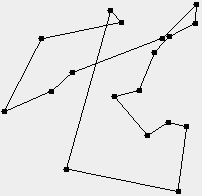
\includegraphics[width=0.48\textwidth]{images/result3/Pathfalse9.png}
        \caption{Rank selection.}
        \label{fig:cities18GraphPathfalse}
    \end{subfigure}
    \begin{subfigure}[b]{0.23\textwidth}
        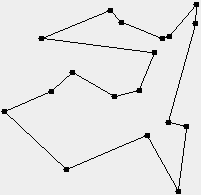
\includegraphics[width=0.48\textwidth]{images/result3/Pathtrue2.png}
        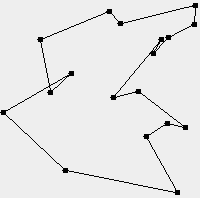
\includegraphics[width=0.48\textwidth]{images/result3/Pathtrue4.png}
        \caption{MRS}
        \label{fig:cities18GraphPathtrue}
    \end{subfigure}  
    \caption{Path representation}
    \label{fig:cities18GraphPath}
\end{center}
\end{figure}

\noindent During the experiments involving 10 and 15 cities the multi-reserved strategy has converged on a shorter tour than the rank selection. When 18 cities are used we see this flip and rank selection starts to find shorter tours. This will be discussed further in the experiments that involve 20 cities. \\


\begin{table}[H]
\centering
\begin{tabular}{|c|c|c|c|c|c|c|}
\hline
\multicolumn{1}{|l|}{\multirow{2}{*}{\textbf{Rep.}}} & \multicolumn{1}{l|}{\multirow{2}{*}{\textbf{Sel.}}} & \multicolumn{1}{l|}{\multirow{2}{*}{\textbf{Gen.}}} & \multicolumn{3}{c|}{\textbf{In final generation}}                                                                & \multicolumn{1}{l|}{\multirow{2}{*}{\textbf{F.}}} \\ \cline{4-6}
\multicolumn{1}{|l|}{}                               & \multicolumn{1}{l|}{}                               & \multicolumn{1}{l|}{}                               & \multicolumn{1}{l|}{\textbf{Avg.}} & \multicolumn{1}{l|}{\textbf{Least}} & \multicolumn{1}{l|}{\textbf{F.}} & \multicolumn{1}{l|}{}                                  \\ \hline
\multirow{2}{*}{B.}                                  & Rank                                                & 4613                                                & 1070                               & 1519                                & 1065                                  & 1065                                                   \\ \cline{2-7} 
                                                     & MRS                                                & 1961                                                & 1231                               & 1941                                & 1179                                  & 1179                                                   \\ \hline
\multirow{2}{*}{P.}                                  & Rank                                                & 318                                                 & 915                                & 1092                                 & 914                                   & 913                                                    \\ \cline{2-7} 
                                                     & MRS                                                & 400                                                 & 1007                                & 1361                                & 997                                   & 997                                                    \\ \hline
\end{tabular}
\caption{Number of cities : 18, Population size : 500}
\label{table:18cities}
\end{table}

\noindent \textit{20 cities} \\

\noindent The next experiments explore what happens when the number of cities in increased to 20. Just like the experiments with 15 and 18 cities, the path representation has found shorter tours and taken fewer iterations than binary representation. \\

\noindent When using binary representation the rank selection reached the maximum number of generations. There has been no change in the fitness of the fittest individual for many generations, but as the least fittest individual changes rapidly so does the average fitness. This causes the GA to converge slowly. (Shown in figure~\ref{fig:cities20GraphBinaryfalse}.) \\


\begin{table}[H]
\centering
\begin{tabular}{|c|c|c|c|c|c|c|}
\hline
\multicolumn{1}{|l|}{\multirow{2}{*}{\textbf{Rep.}}} & \multicolumn{1}{l|}{\multirow{2}{*}{\textbf{Sel.}}} & \multicolumn{1}{l|}{\multirow{2}{*}{\textbf{Gen.}}} & \multicolumn{3}{c|}{\textbf{In final generation}}                                                                & \multicolumn{1}{l|}{\multirow{2}{*}{\textbf{F.}}} \\ \cline{4-6}
\multicolumn{1}{|l|}{}                               & \multicolumn{1}{l|}{}                               & \multicolumn{1}{l|}{}                               & \multicolumn{1}{l|}{\textbf{Avg.}} & \multicolumn{1}{l|}{\textbf{Least}} & \multicolumn{1}{l|}{\textbf{F.}} & \multicolumn{1}{l|}{}                                  \\ \hline
\multirow{2}{*}{B.}                                  & Rank                                                & 5000                                                & 1199                               & 2066                                & 1191                                  & 1191                                                   \\ \cline{2-7} 
                                                     & MRS                                                & 1623                                                & 1289                               & 2361                                & 1218                                  & 1218                                                   \\ \hline
\multirow{2}{*}{P.}                                  & Rank                                                & 627                                                 & 935                               & 1297                                & 933                                  & 933                                                   \\ \cline{2-7} 
                                                     & MRS                                                & 575                                                 & 997                                & 1481                                & 985                                   & 985                                                    \\ \hline
\end{tabular}
\caption{Number of cities : 20, Population size : 1000}
\label{table:20cities}
\end{table}

\noindent The mutation and crossover could be having a larger effect on the tours produced by the binary representation than the path representation. Changing the more significant bits of the binary representation can completely change the tour. When fewer cities are used the effect of this is less noticeable. Therefore, in the experiment with just 10 cities the results were very similar, but with 20 cities we see a large difference. These large changes will prevent local area search. \\


\noindent As individuals change a lot this causes the average fitness to remain unstable, so the GA will take longer to converge. This can be see in figure~\ref{fig:cities20GraphBinarytrue}. The GA has only converged because the average fitness has risen for more than 10 generations. Though the least fit individual's fitness does fall slightly at the start, in comparison to the path representation (figures~\ref{fig:cities20GraphPathtrue} and~\ref{fig:cities20GraphPathfalse}) there is a greater difference between this and the average fitness.\\



\begin{figure}[H]
\begin{center}
    \begin{subfigure}[b]{0.24\textwidth}
    \begin{minipage}{\textwidth}\footnotesize

  		\subsubfloat{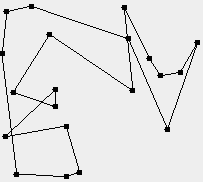
\includegraphics[width=0.48\textwidth]{images/result4/Binaryfalse0.png}}{Rank selection}\label{fig:cities20toursBR}
  		\subsubfloat{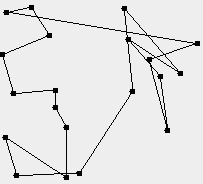
\includegraphics[width=0.48\textwidth]{images/result4/Binarytrue2.png}}{MRS}\label{fig:cities20toursOM}
 	\caption{Binary representation}\label{fig:cities20toursB}
  \end{minipage}
        
    \end{subfigure}
    \begin{subfigure}[b]{0.24\textwidth}
    \begin{minipage}{\textwidth}\footnotesize

  		\subsubfloat{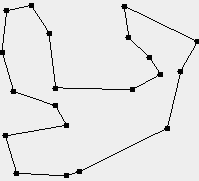
\includegraphics[width=0.48\textwidth]{images/result4/Pathfalse3.png}}{Rank selection}\label{fig:cities20toursOR}
  		\subsubfloat{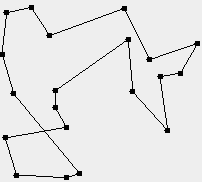
\includegraphics[width=0.48\textwidth]{images/result4/Pathtrue9.png}}{MRS}\label{fig:cities20toursOM}
 		\caption{Path representation}\label{fig:cities20toursO}
  \end{minipage}
        
    \end{subfigure} 
    \caption{Selection of tours produced for 20 cities}
    \label{fig:cities20tours}
\end{center}
\end{figure}


\noindent In contrast to previous experiments the rank selection has out performed the multi-reserved strategy, but only a small difference is seen. From one experiment it was unclear if any conclusions could be drawn. Therefore, the experiments with 20 cities were run using several different city positions. There appears to be a 50/50 chance of multi-reserved strategy converging to a shorter tour than rank selection. Therefore, no clear conclusion can be drawn between which selection operator is better at solving a 20 city TSP.\\

\begin{figure}[H]
\begin{center}
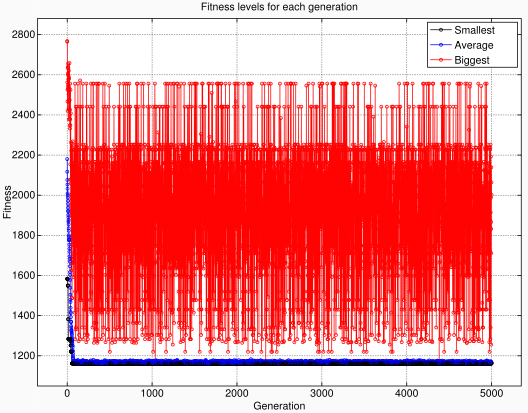
\includegraphics[scale=0.4]{images/result4/GraphBinaryfalse0.png} 
\caption{Binary representation using rank selection.}
\label{fig:cities20GraphBinaryfalse}
\end{center}
\end{figure}

\begin{figure}[H]
\begin{center}
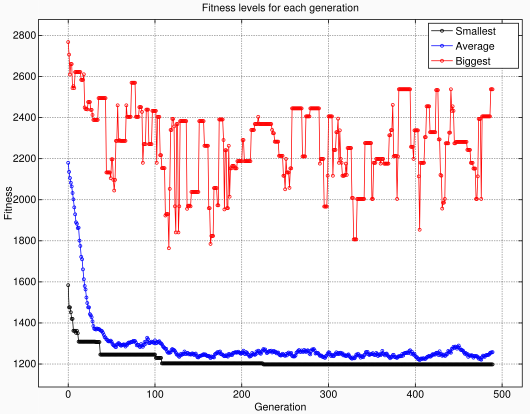
\includegraphics[scale=0.4]{images/result4/GraphBinarytrue2.png} 
\caption{Binary representation using  MRS.}
\label{fig:cities20GraphBinarytrue}
\end{center}
\end{figure}


\begin{figure}[H]
\begin{center}
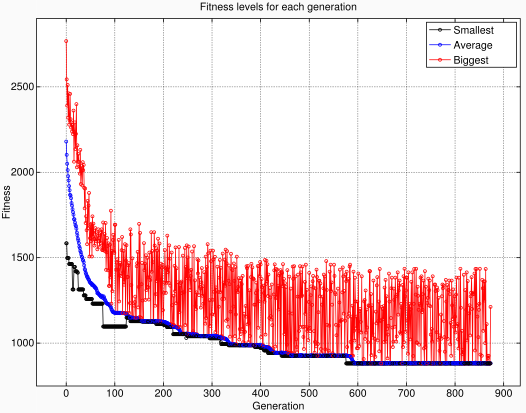
\includegraphics[scale=0.4]{images/result4/GraphPathfalse3.png} 
\caption{Path representation using rank selection.}
\label{fig:cities20GraphPathfalse}
\end{center}
\end{figure}

\begin{figure}[H]
\begin{center}
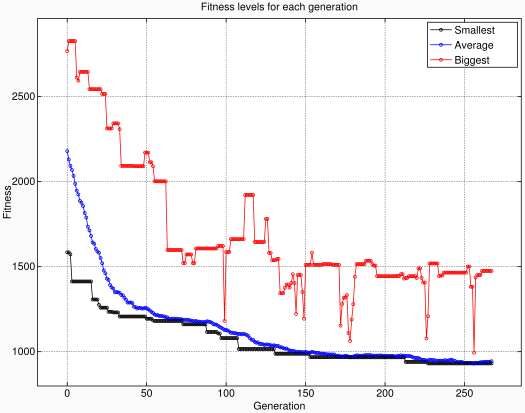
\includegraphics[scale=0.4]{images/result4/GraphPathtrue9.png} 
\caption{Path representation using MRS.}
\label{fig:cities20GraphPathtrue}
\end{center}
\end{figure}

\noindent Overtime the path representation least fittest, fittest and average fitness has fallen steeply before levelling off. The least fittest line shows that the genetic operations have allowed variations in the tours to enter the population. This helps local minims to be escaped. Though the algorithm can still fall into minims, often a correct, or close to correct, tour is discovered.\\


\subsubsection{Experiment Summary}

The number of generations needed before the GA converges is greater for binary representation than path representation. When the average fitness of a generation does not fall for 10 generations then the GA stops. The average fitness remains far less stable in the binary representation (figure~\ref{fig:cities20GraphBinarytrue}) than in the path representation (figure~\ref{fig:cities20GraphPathtrue}). It is likely that the mutation probability has been set too high causing too much change in the individuals. \\

\noindent Each experiment was run 10 times and the averages of these were used when discussing the results. However, during these 10 runs a wide range in the number of generations was seen. For the experiment on 20 cities using path representation with rank selection the number of generations ranged from 153 to 1035. When the number of generations reached 1035 the last drop in the fittest individual was seen around the 350th generation. Therefore perhaps an alternative stopping criteria should have been used. For example it could be based on the number of generations where the fittest individual has not changed.\\

\noindent As more cities are added the tours discovered by the binary representation quickly become far worse. Whereas, the path representation becomes worse at a much slower rate and can still sometimes find the shortest tour. Experiments with large numbers of cities were performed and these experiments continued to become less likely to find the shortest tour.  \\

\noindent The experiments have shown that, for the genetic operations chosen, path representation finds a shorter tour and uses less generations, than binary representation. The multi-reserved strategy takes more generations to converge than the rank selection, however similar tour lengths are found.

\subsubsection{Improvements to experiments}
Rather than using a value for mutation and crossover probability that is in the form of $1 / p$, a value in the range 0 to 1 should have been used. This would make it more user friendly as 0 would cause no mutation/crossover to take place; and 1 would cause every binary value, or ordered list, to mutate/crossover. This should not impact the validity of the results produced. \\

\section{Conclusion}

\subsection{Future experiments with GAs}
Experiments using the binary representation with different types of crossover operations could be performed. One-point crossover causes a large change to the individuals, which prevents local area being searched. Using two-point crossover may allow a shorter tours to be discovered.\\

\noindent The GA produced checks that no individuals are the same within a single generation, but it does not check that the individuals are unique within the life time of the GA. These means that the fitness function is potentially being ran many times using the same input. Future work could consider remembering the fitness. This will add a large memory overhead, but may save on computational time.\\

\noindent The initial population produced may not be distributed across a wide area of the search space. This may cause the population to be trapped within a local search area. Experiments using a Gaussian or Bernoulli distribution could be performed.\\

\noindent The experiments used show that when using path representation there is a good chance that the shortest tour will be found. However as more cities are added this becomes less and less likely. The GA is likely to discover a local minim. Alternative methods for solving TSP should be considered. 

\subsection{Alternative methods}

Swarm intelligence would  allow a large area of the search space to be explored and individuals would be able to adapt according to how other individuals perform. This should lead to all individuals converging of the minim value. There are many forms of swarm intelligence including Ant Colony Optimization (ACO) and Particle Swarm Optimization (PSO).\\

\noindent Chen et. al. \cite{swarmIntelligence} has compared their method, Gene Regulation Particle Swarm Ant Colony Optimization (GRPSAC), to ACO, PSO and a GA to find out which method is better at solving the TSP. Their results show that for 30 cities ACO achieves the worst solutions, followed by GAs. When using 48 cites the GA, on average, has the worst results.\\

\noindent Chen et. al., and related work, has shown that swarm intelligence can perform much better at solving TSP than GAs. Therefore, further research such look at adapting and improving swarm intelligence methods in order to achieve more optimal solutions for the TSP.


\end{multicols}
\nocite{*}
\bibliographystyle{plain}
\bibliography{references}

\end{document}